\documentclass[11pt]{article}
\usepackage{textcomp}
\usepackage{fontenc}

\usepackage{graphicx}
\usepackage{caption}
\usepackage{sidecap}
\usepackage{enumitem}
\usepackage{multicol}
\usepackage{gensymb}
\usepackage{placeins}
\setlength{\parskip}{3 mm}

\graphicspath{{images/}}	% Root directory of the figures

\title{Community Dyanmics meta analysis - Draft}

\renewcommand*{\familydefault}{\sfdefault}



\begin{document}

\maketitle
% \section{Abstract}


% \section{Introduction}

% \section{Materials and Methods}


\section{Results}


Overall relationship between spatial and temporal heterogeneity

Dispersion (spatial heterogeneity) is the single largest factor in driving temporal heterogeneity. Lifespan of organism, spatial extent, time step, biome all exert only weak effects on this relationship. Spatial heterogeneity is related to evenness at site and plot level. 

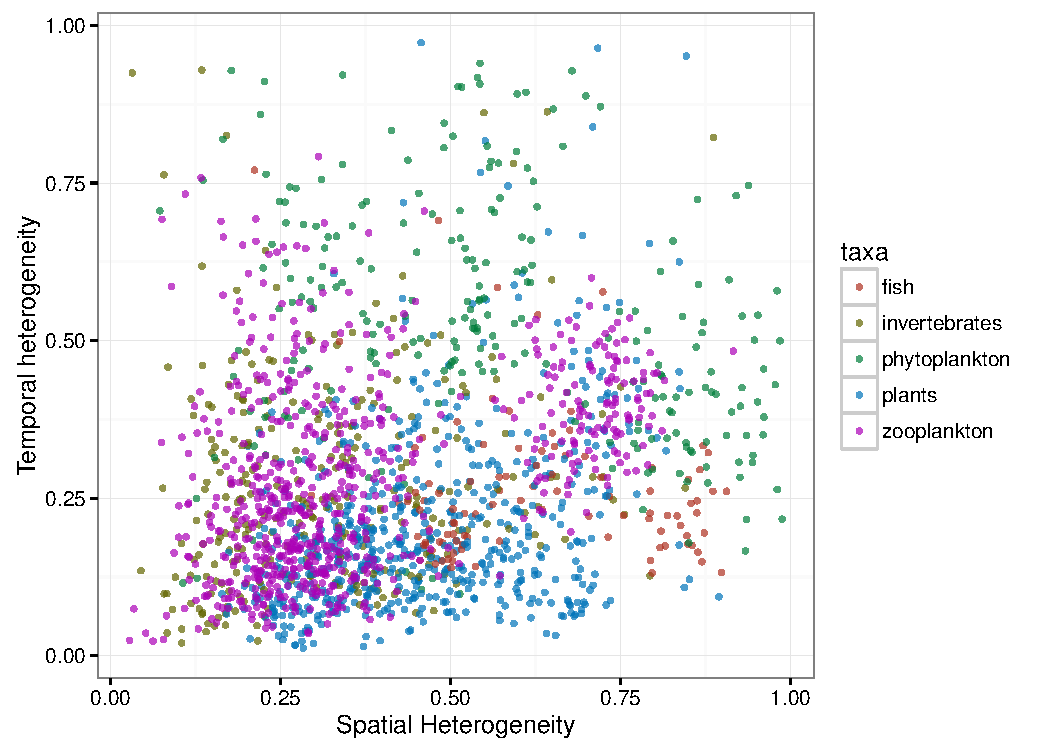
\includegraphics[width=400px]{overall}


\newpage
Overall relationship, aggregated by study.

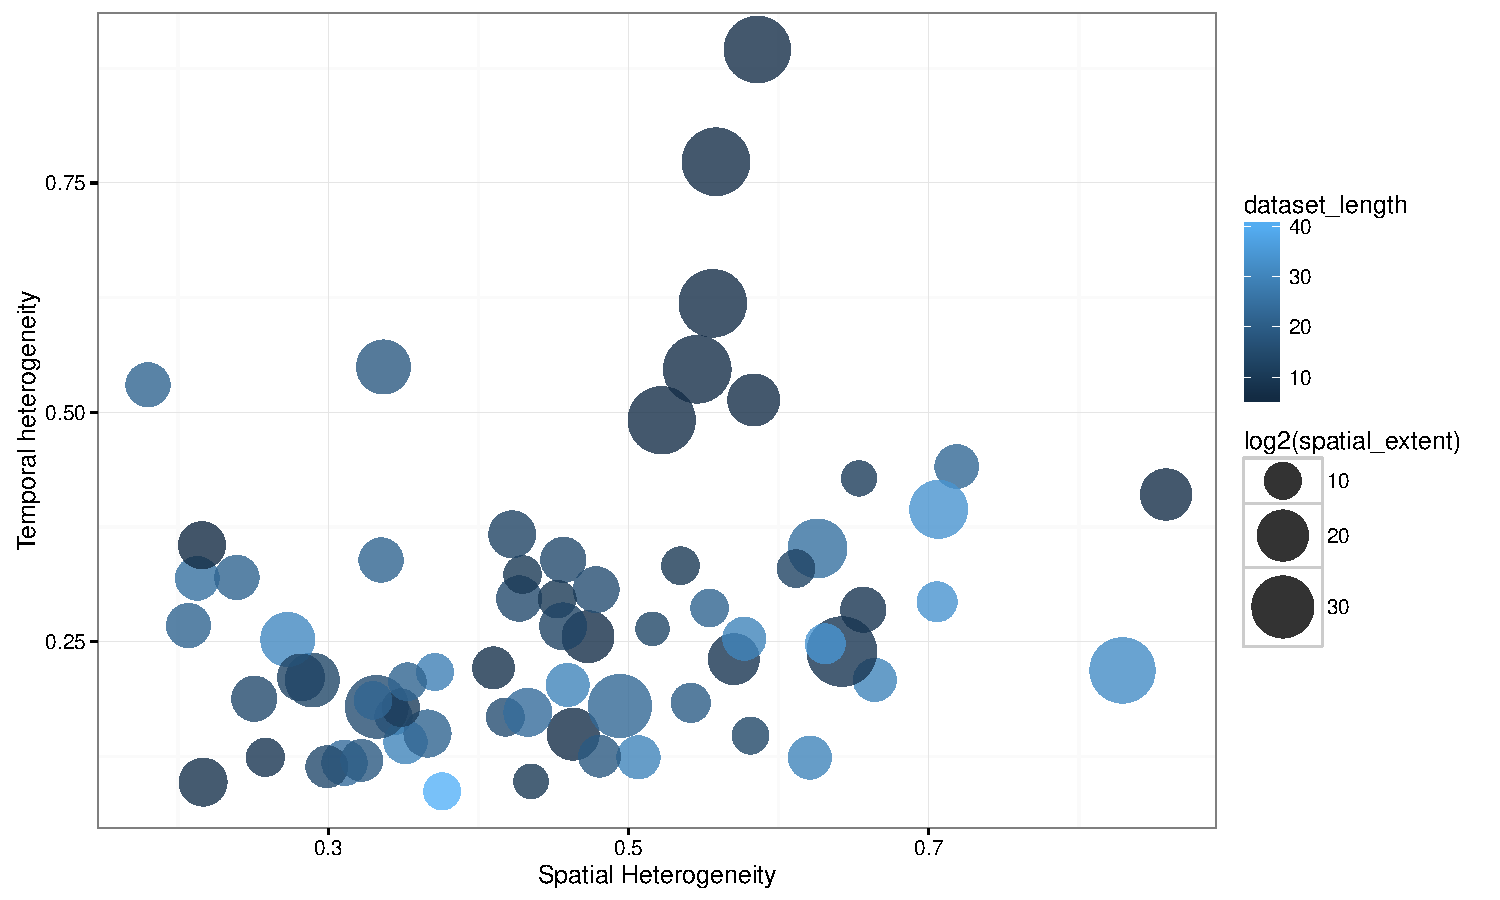
\includegraphics[width=400px]{overallagg}


\newpage
Difference between aquatic and terrestrial studies

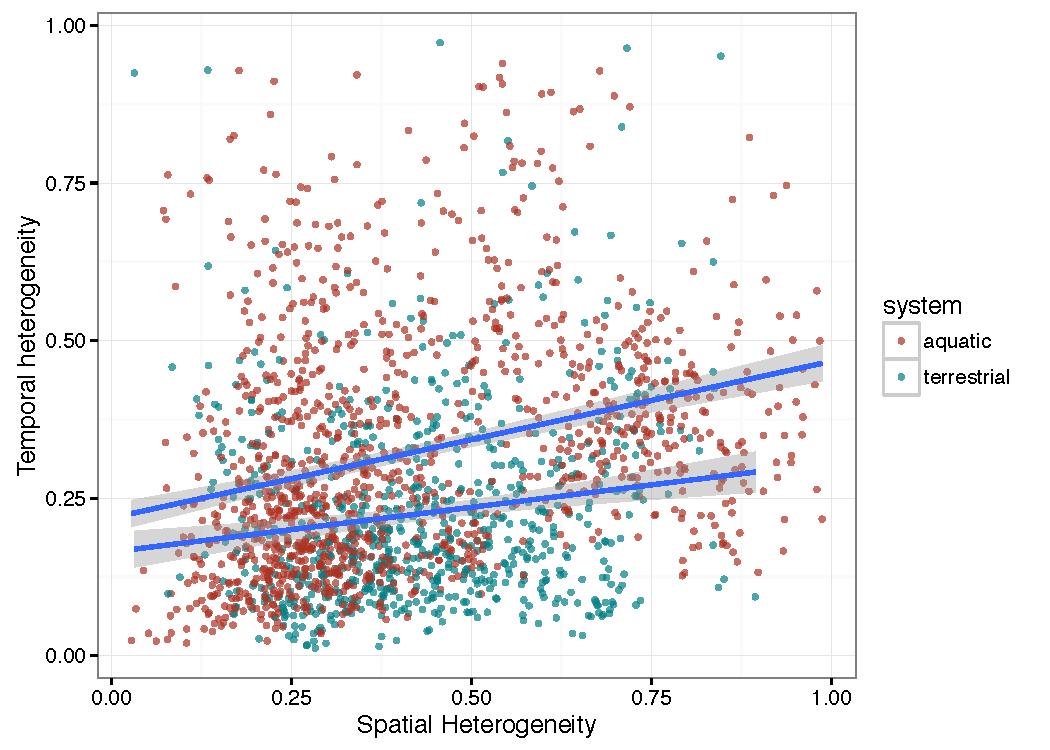
\includegraphics[width=400px]{aqterr}
\newpage

Table 1. Summary of mixed effect model of spatial heterogeneity on temporal heterogeneity, with study design features as covariates

\FloatBarrier
\begin{table}[ht]
\centering
\begin{tabular}{rrrr}
  \hline
 & Estimate & Std. Error & t value \\ 
  \hline
(Intercept) & 0.29 & 0.07 & 4.00 \\ 
  dispersion & 0.23 & 0.08 & 3.00 \\ 
  plot\_size & -0.00 & 0.00 & -0.66 \\ 
  num\_plots & 0.00 & 0.00 & 0.73 \\ 
  spatial\_extent & -0.00 & 0.00 & -0.37 \\ 
  dataset\_length & -0.00 & 0.00 & -1.79 \\ 
  time\_step & -0.07 & 0.04 & -1.67 \\ 
   \hline
\end{tabular}
\end{table}
\FloatBarrier



Figure 4. Summary of mixed-effect model for study design features 

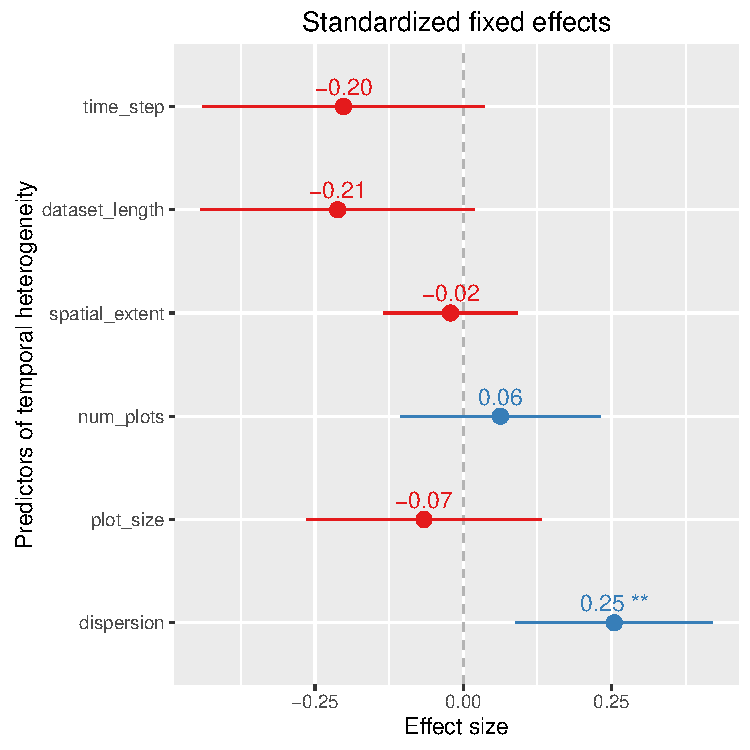
\includegraphics[width=300px]{designmodel}
\pagebreak


Table 2. System and organism-level features as covariates of effect of spatial heterogeneity on temporal heterogeneity

\FloatBarrier
\begin{table}[ht]
\centering
\begin{tabular}{rrrr}
  \hline
 & Estimate & Std. Error & t value \\ 
  \hline
(Intercept) & 0.05 & 0.15 & 0.35 \\ 
  dispersion & 0.33 & 0.08 & 3.99 \\ 
  taxainvertebrates & 0.16 & 0.17 & 0.95 \\ 
  taxaphytoplankton & 0.18 & 0.17 & 1.03 \\ 
  taxaplants & 0.12 & 0.17 & 0.72 \\ 
  taxazooplankton & 0.12 & 0.15 & 0.78 \\ 
  lifespanlonger & -0.07 & 0.04 & -1.62 \\ 
  S & 0.00 & 0.00 & 0.64 \\ 
  ANPP & -0.00 & 0.00 & -0.43 \\ 
  successionyes & 0.05 & 0.03 & 1.84 \\ 
  systemterrestrial & -0.06 & 0.10 & -0.55 \\ 
   \hline
\end{tabular}
\end{table}
\FloatBarrier


Figure 5. Summary of mixed-effect model for taxonomic and ecosystem type system features 

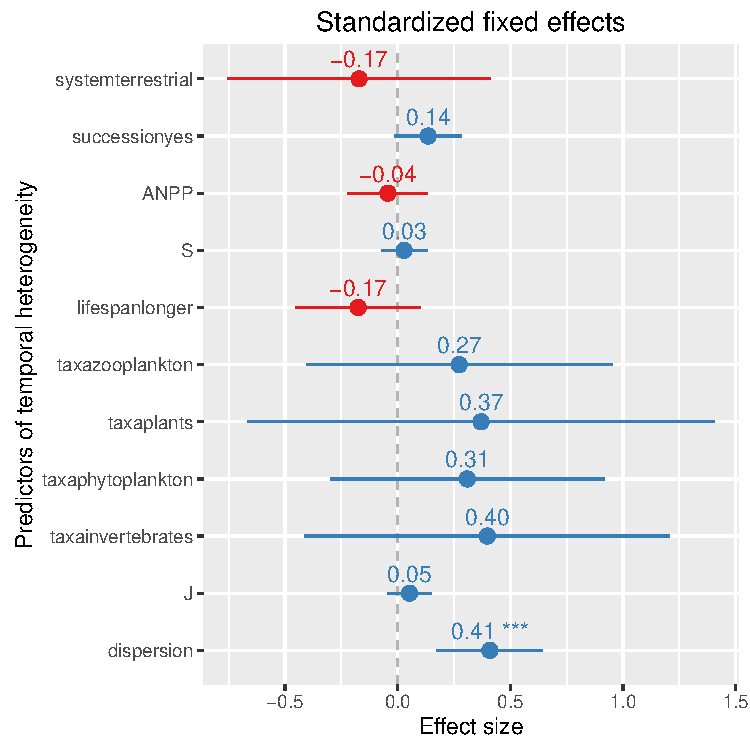
\includegraphics[width=280px]{systemmodel}


Table 3. Interaction between plot-level evenness, site-level evenness, and dispersion. There is an interaction between dispersion and evenness, such that including effects of plot-level evenness and site-level evenness does reduce the predictive power of dispersion itself, when no other factors are included. 

\FloatBarrier
\begin{table}[ht]
\centering
\begin{tabular}{rrrr}
  \hline
 & Estimate & Std. Error & t value \\ 
  \hline
(Intercept) & 0.13 & 0.06 & 2.05 \\ 
  dispersion & 0.14 & 0.15 & 0.99 \\ 
  J & -0.03 & 0.19 & -0.16 \\ 
  plotJ & 0.13 & 0.18 & 0.72 \\ 
  dispersion:J & 0.15 & 0.37 & 0.39 \\ 
  dispersion:plotJ & -0.12 & 0.32 & -0.38 \\ 
   \hline
\end{tabular}
\end{table}
\FloatBarrier

Figure 6. Interaction model

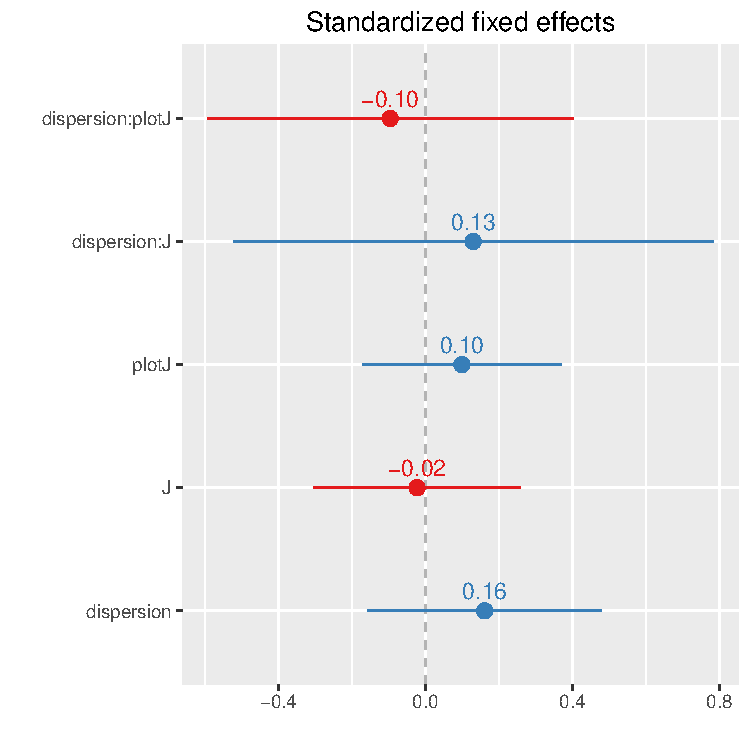
\includegraphics[width=280px]{interaxplot}

Using presence-absence based measure of both temporal and spatial heterogeneity, results are the same

\FloatBarrier
\begin{table}[ht]
\centering
\begin{tabular}{rrrr}
  \hline
 & Estimate & Std. Error & t value \\ 
  \hline
(Intercept) & 0.09 & 0.12 & 0.73 \\ 
  jac\_disp & 0.56 & 0.16 & 3.38 \\ 
  S & -0.00 & 0.00 & -3.85 \\ 
  J & -0.15 & 0.03 & -5.88 \\ 
   \hline
\end{tabular}
\end{table}
\FloatBarrier

Figure 7. Presence-absence model

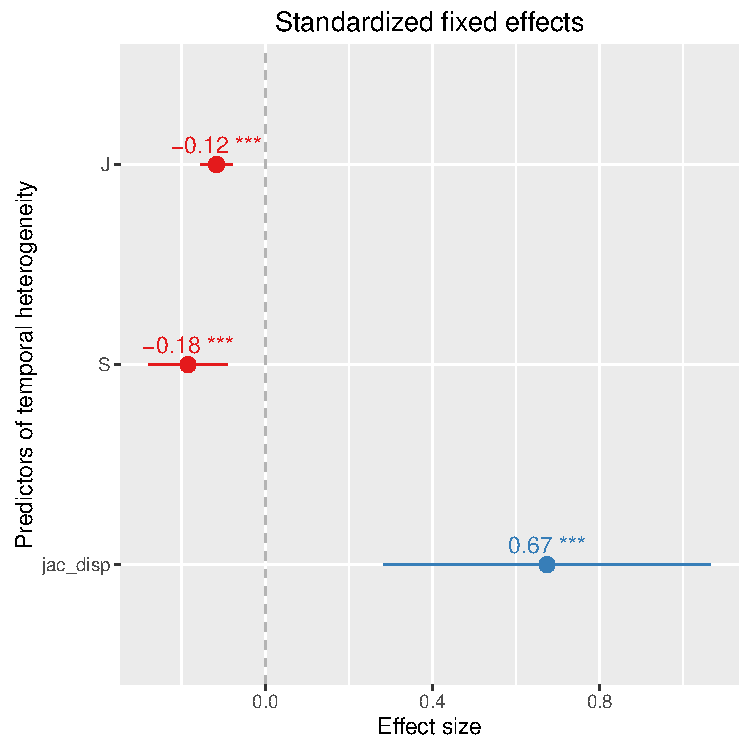
\includegraphics[width=280px]{pa-evenness}


Map of data sources: All

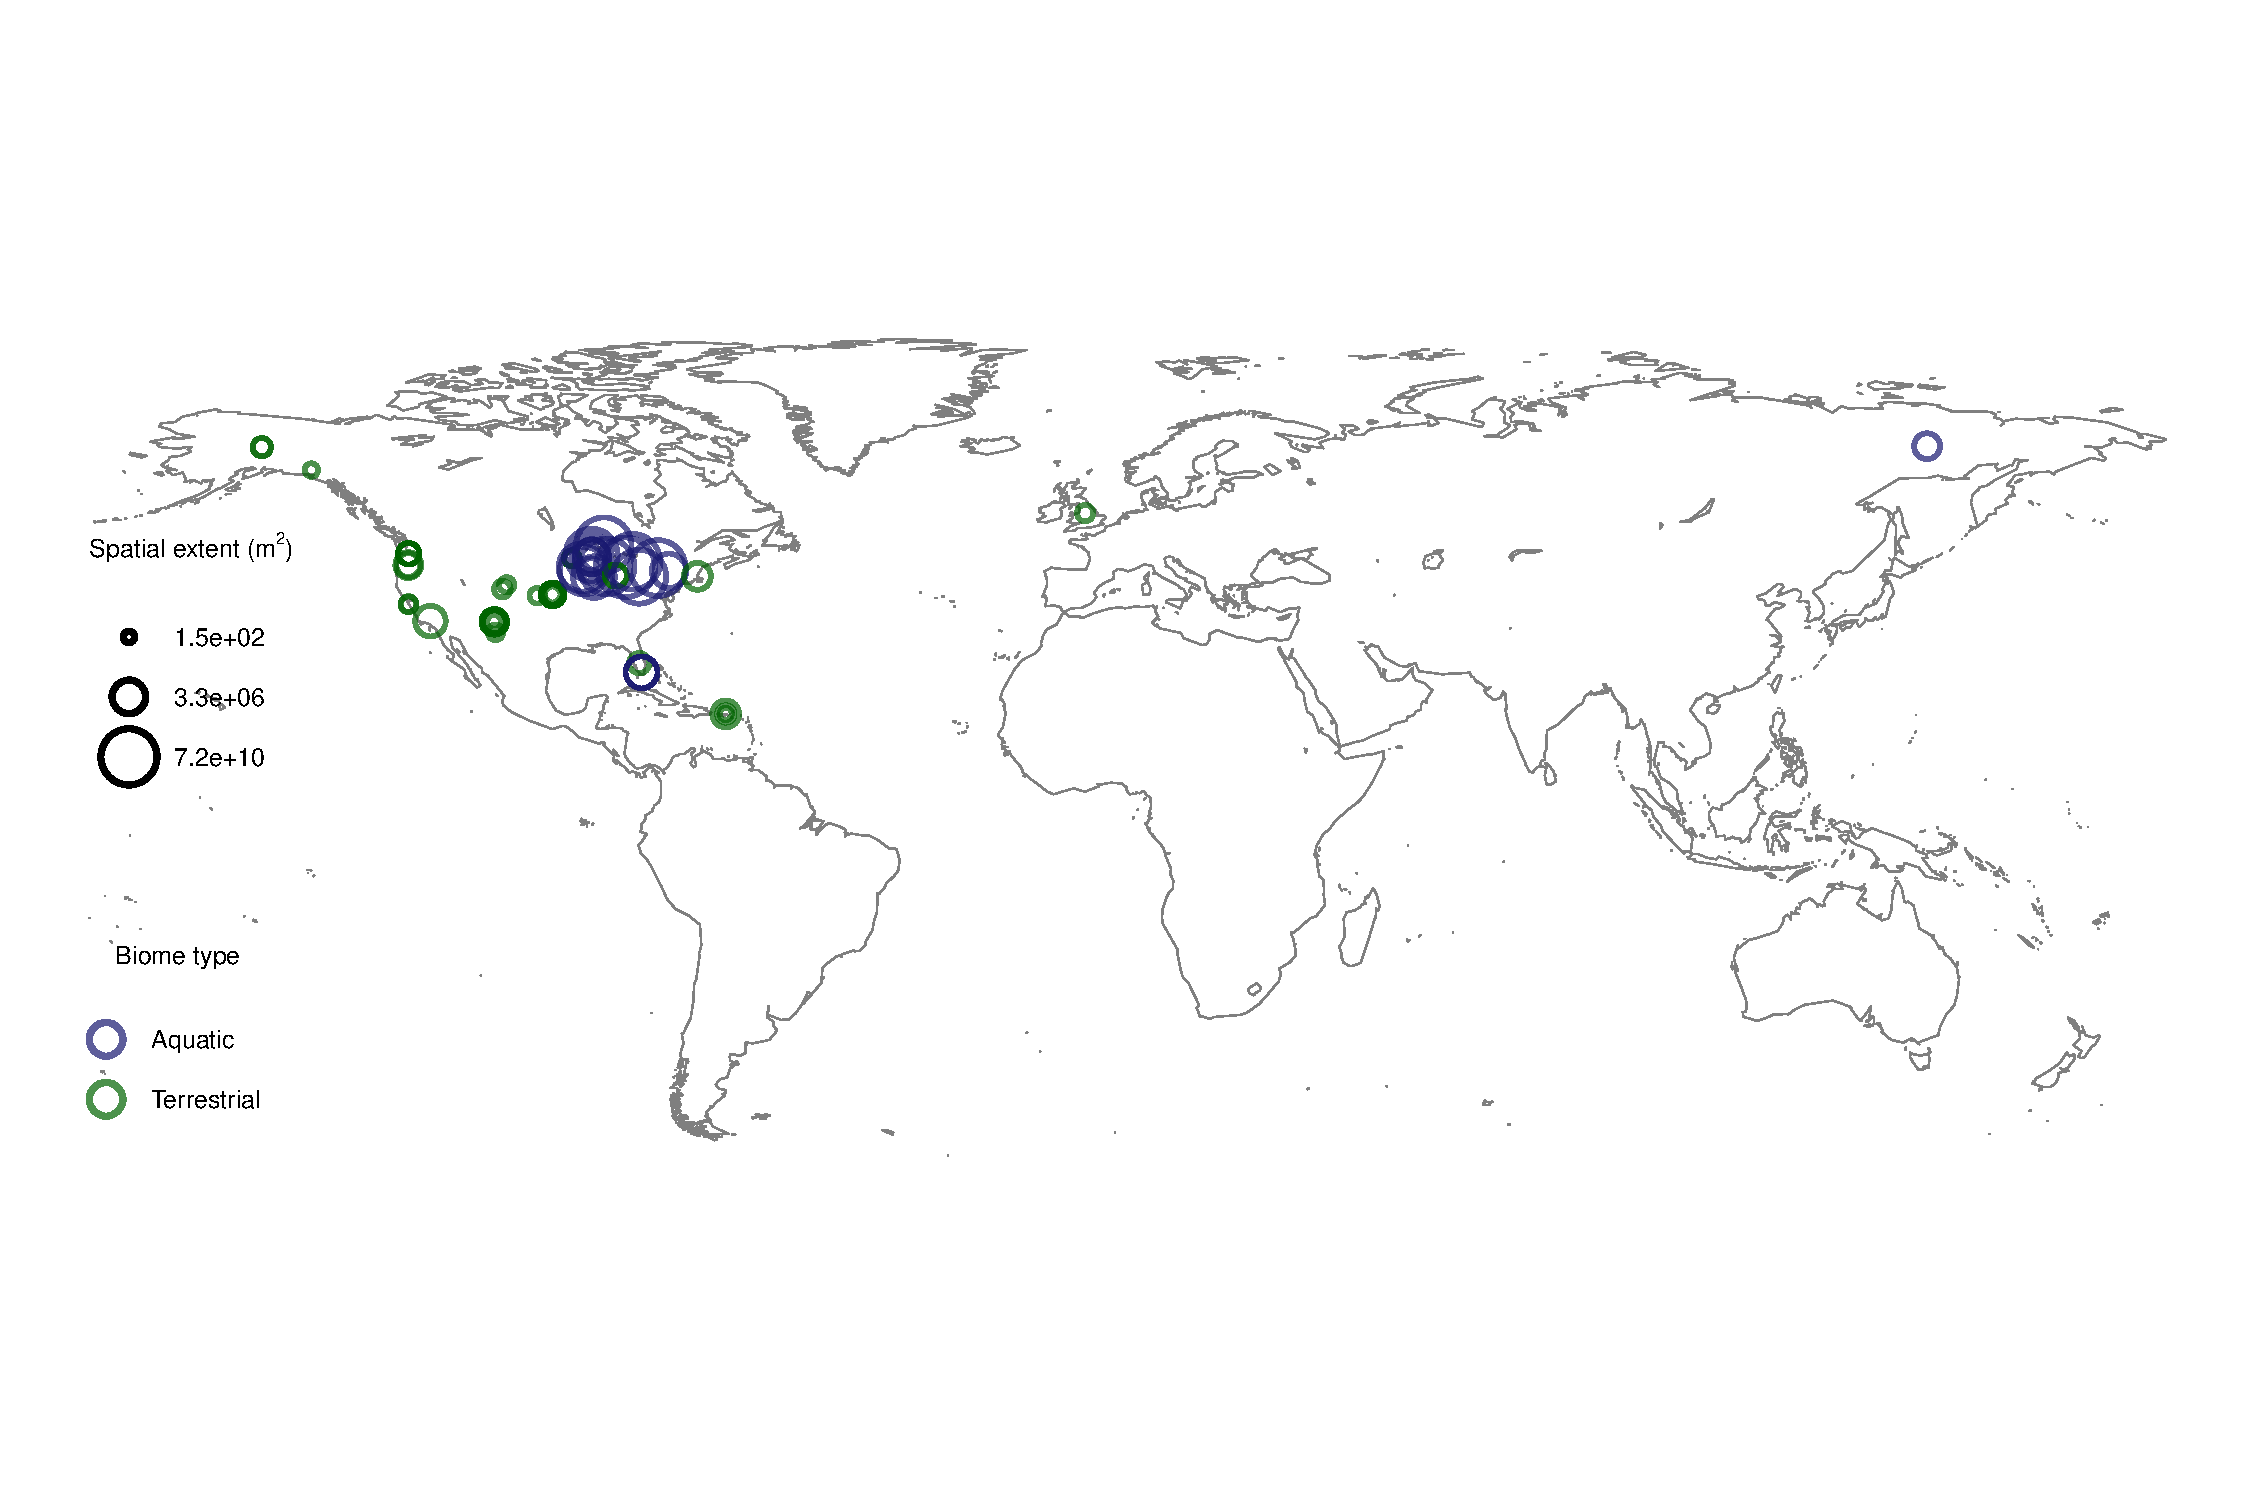
\includegraphics[width=450px]{BigMap}

Map of data sources: North America only

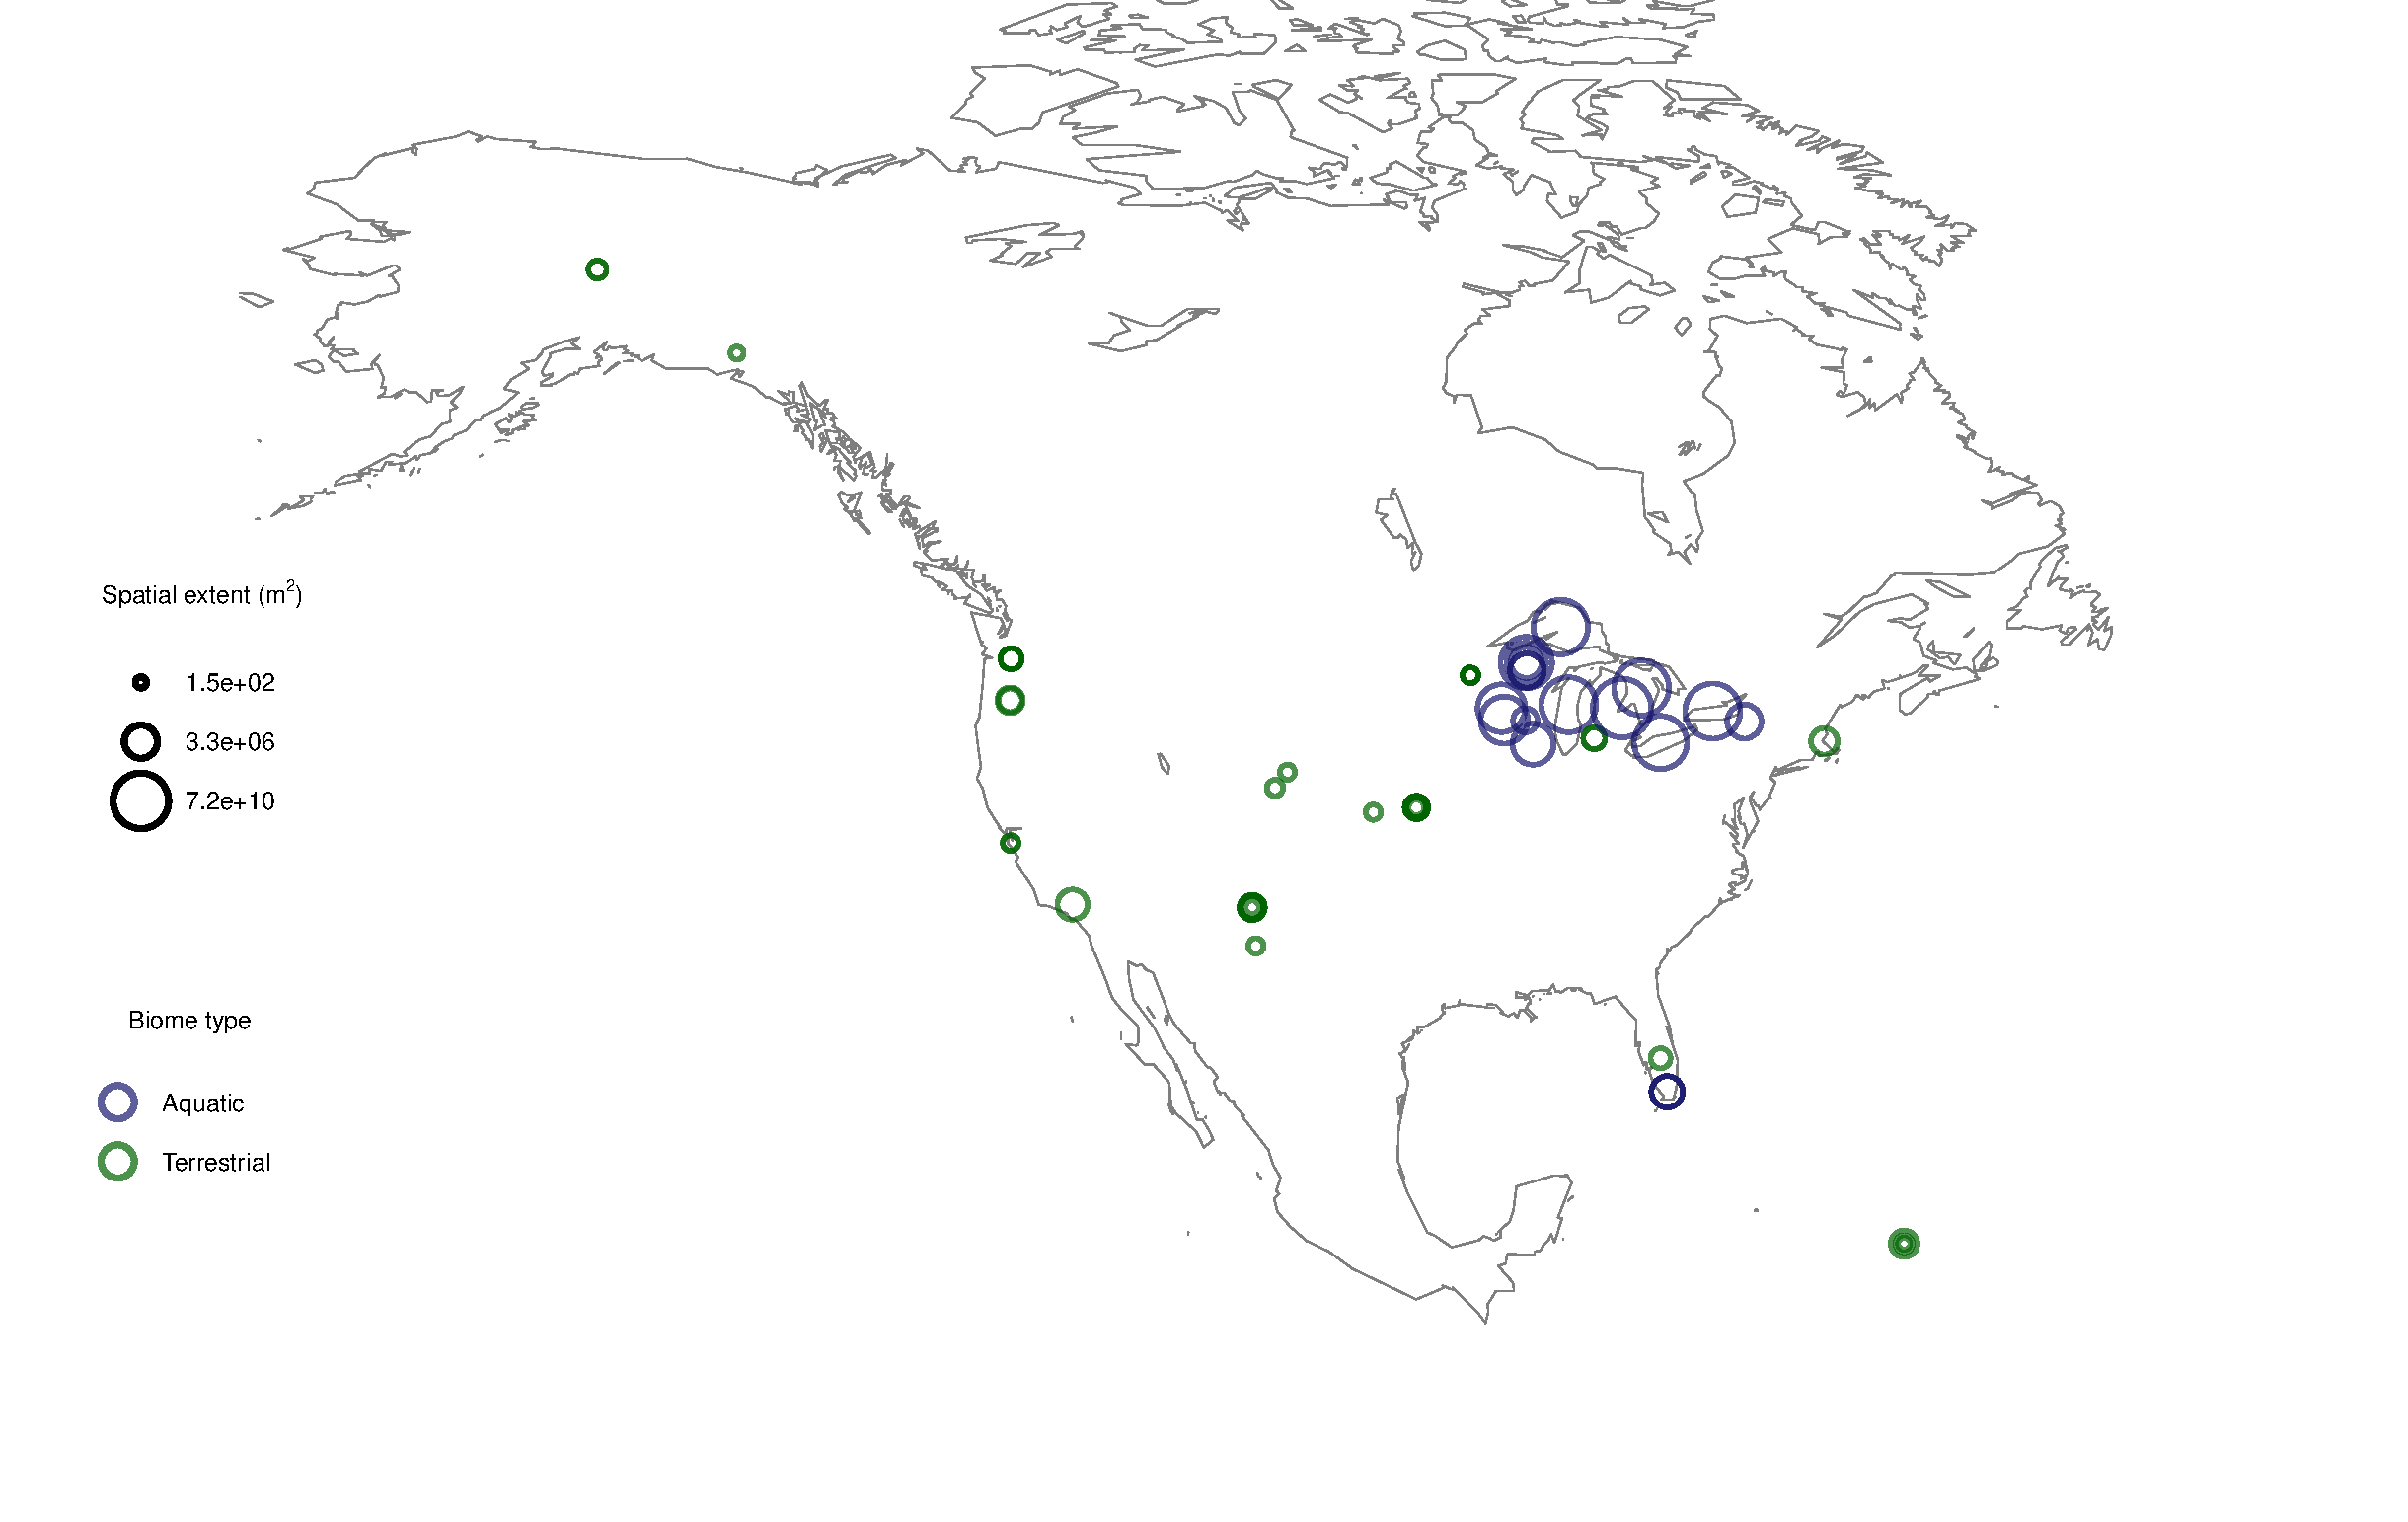
\includegraphics[width=450px]{NAmap1}



\end{document}